\begin{equation*}
% the traversal takes the site's --mred (#7a2518): its walk on the left, the entries it uses on the right
\definecolor{lanecolor}{RGB}{122,37,24}%
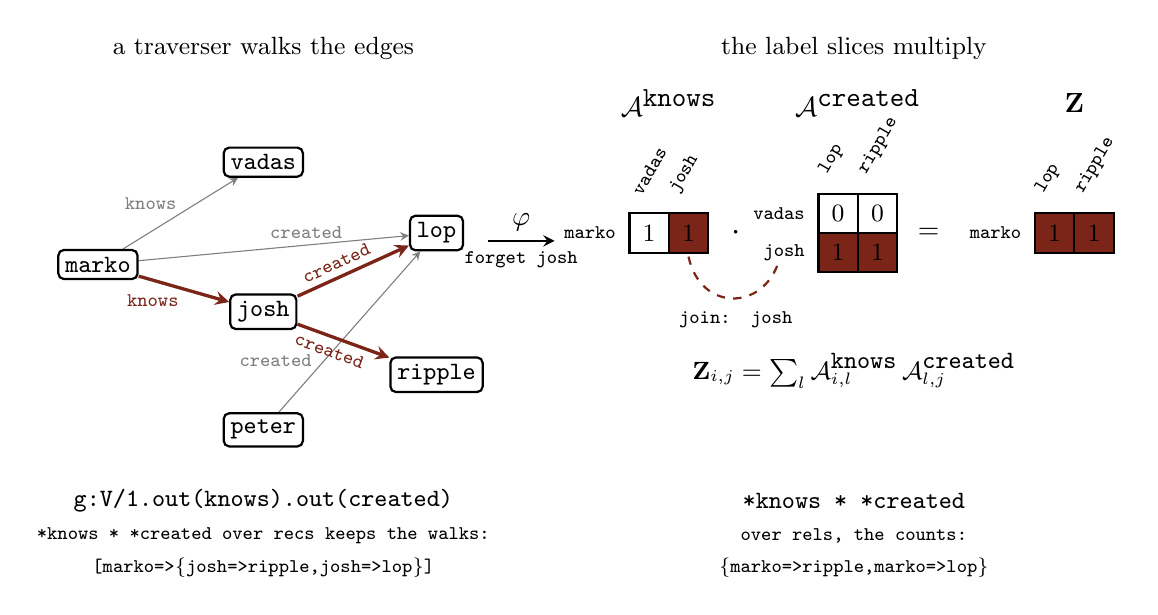
\begin{tikzpicture}[
  vertex/.style={draw, rounded corners=2pt, thick, font=\small\ttfamily, inner sep=2.5pt},
  edge/.style={thin, ->, >=stealth, opacity=0.5},
  lane/.style={very thick, ->, >=stealth, color=lanecolor},
  elabel/.style={font=\scriptsize\ttfamily},
  cell/.style={draw, thick, minimum size=5mm, inner sep=0pt, font=\small},
  hot/.style={cell, fill=lanecolor},
  axis/.style={font=\scriptsize\ttfamily},
  note/.style={font=\small}
]
% ---- the network: a traverser walks the edges ----
\node[note] at (2.1, 2.75) {a traverser walks the edges};
\node[vertex] (marko)  at (0, 0)      {marko};
\node[vertex] (vadas)  at (2.1, 1.3)  {vadas};
\node[vertex] (josh)   at (2.1, -0.6) {josh};
\node[vertex] (peter)  at (2.1, -2.1) {peter};
\node[vertex] (lop)    at (4.3, 0.4)  {lop};
\node[vertex] (ripple) at (4.3, -1.4) {ripple};
\draw[edge] (marko) -- node[elabel, above left=-2pt] {knows} (vadas);
\draw[edge] (marko) -- node[elabel, above=-1pt, pos=0.62] {created} (lop);
\draw[edge] (peter) -- node[elabel, left=1pt, pos=0.32] {created} (lop);
\draw[lane] (marko) -- node[elabel, below left=-2pt] {knows} (josh);
\draw[lane] (josh) -- node[elabel, above=-1pt, pos=0.4, sloped] {created} (lop);
\draw[lane] (josh) -- node[elabel, below=-1pt, pos=0.4, sloped] {created} (ripple);
% ---- phi: the walks onto the counts ----
\draw[thick, ->, >=stealth] (4.95, 0.3) -- node[above] {$\varphi$} node[elabel, below] {forget josh} (5.8, 0.3);
% ---- the matrix: the label slices multiply ----
\node[note] at (9.6, 2.75) {the label slices multiply};
% A^knows: the row of marko, the columns of vadas and josh
\node at (7.25, 2.05) {$\mathcal{A}^{\texttt{knows}}$};
\node[cell] at (7.0, 0.4) {$1$};
\node[hot]  at (7.5, 0.4) {$1$};
\node[axis, anchor=east] at (6.7, 0.4) {marko};
\node[axis, anchor=south west, rotate=60] at (6.95, 0.7) {vadas};
\node[axis, anchor=south west, rotate=60] at (7.45, 0.7) {josh};
\node[font=\large] at (8.1, 0.4) {$\cdot$};
% A^created: the rows of vadas and josh, the columns of lop and ripple
\node at (9.65, 2.05) {$\mathcal{A}^{\texttt{created}}$};
\node[cell] at (9.4, 0.65)  {$0$};
\node[cell] at (9.9, 0.65)  {$0$};
\node[hot]  at (9.4, 0.15)  {$1$};
\node[hot]  at (9.9, 0.15)  {$1$};
\node[axis, anchor=east] at (9.1, 0.65) {vadas};
\node[axis, anchor=east] at (9.1, 0.15) {josh};
\node[axis, anchor=south west, rotate=60] at (9.35, 0.95) {lop};
\node[axis, anchor=south west, rotate=60] at (9.85, 0.95) {ripple};
\node at (10.55, 0.4) {$=$};
% Z: the row of marko, the columns of lop and ripple, each a count of walks
\node at (12.4, 2.05) {$\mathbf{Z}$};
\node[hot] at (12.15, 0.4) {$1$};
\node[hot] at (12.65, 0.4) {$1$};
\node[axis, anchor=east] at (11.85, 0.4) {marko};
\node[axis, anchor=south west, rotate=60] at (12.1, 0.7) {lop};
\node[axis, anchor=south west, rotate=60] at (12.6, 0.7) {ripple};
% the join vertex: josh's column meets josh's row, and the product sums it away
\draw[thick, dashed, color=lanecolor] (7.5, 0.1) .. controls (7.65, -0.6) and (8.45, -0.6) .. (8.65, 0.05);
\node[elabel] at (8.1, -0.7) {join: josh};
\node[note] at (9.6, -1.35) {$\mathbf{Z}_{i,j} = \sum_{l} \mathcal{A}^{\texttt{knows}}_{i,l}\,\mathcal{A}^{\texttt{created}}_{l,j}$};
% ---- the two realizations in mtron ----
\node[font=\small\ttfamily] at (2.1, -3.0) {g:V/1.out(knows).out(created)};
\node[elabel] at (2.1, -3.45) {*knows * *created over recs keeps the walks:};
\node[elabel] at (2.1, -3.85) {[marko=>\{josh=>ripple,josh=>lop\}]};
\node[font=\small\ttfamily] at (9.6, -3.0) {*knows * *created};
\node[elabel] at (9.6, -3.45) {over rels, the counts:};
\node[elabel] at (9.6, -3.85) {\{marko=>ripple,marko=>lop\}};
\end{tikzpicture}
\end{equation*}
